\documentclass[12pt, a4paper]{article} %mostra o tipo do documento
\setlength{\topmargin}{-.5in}
\setlength{\textheight}{9in}
\setlength{\textwidth}{6.3in}
\setlength{\oddsidemargin}{-.125in}
\setlength{\evensidemargin}{-.125in}
\usepackage[brazil]{babel} %permite escrever em português
\usepackage[utf8]{inputenc}
\usepackage[a4paper, textheight=260mm, textwidth=162mm]{geometry} %ajusta as margens
\usepackage[T1]{fontenc} %define a fonte das letras
\usepackage{color} %colore as letras
\usepackage{url} %inclui urls
\usepackage[pdfencoding=unicode]{hyperref} %transforma links em texto comum para clicar
\usepackage{amsmath, amssymb, amsthm, amsfonts} %permite fazer textos matemáticos
\usepackage{float} % permite mover tabelas e figuras para qualquer ponto da página
\usepackage{graphicx} %permite colocar imagens no documento
\setlength\parindent{24pt}

\title{Relatório EP3 - MAC0121}
\date{}
\author{João Gabriel Basi - $\text{N}^\circ$ USP: 9793801}
\begin{document}
\maketitle
\begin{enumerate}
\large
\item[1.]\textbf{O programa}
\normalsize\par
O programa recebe um vetor desordenado de $n$ posições e o ordena usando 3-reversões. Quando é possível ordená-lo, o programa imprime uma sequência de movimentos que o fazem, quando não é possível, o programa imprime "Nao e possivel".\\[0.5cm]
\large
\item[2.]\textbf{As funções}
\normalsize\\[0.5cm]
O programa utiliza uma biblioteca feita por mim com algumas funções auxiliares:
\begin{itemize}
\item $myvector.h$: Tem funções que ajudam no manuseio de vetores e matrizes.
\end{itemize}
A função principal do programa é a $triSort$, que coordena como o vetor será ordenado. Para ordenar vetores com tamanhos ímpares ela utiliza as funções:
\begin{itemize}
\item $pMaior$: Recebe um vetor e seu tamanho e retorna a posição do maior elemento do vetor;
\item $triReversao$: Recebe um vetor, seu tamanho e uma posição e realiza uma 3-reversão na posição fornecida.
\end{itemize}
Já para vetores de tamanhos pares, ela utiliza as funções:
\begin{itemize}
\item $separa$: Recebe um vetor, seu tamanho e dois vetores com metade de seu tamanho e separa os elementos do vetor maior pela paridade de seus índices nos dois vetores menores;
\item $junta$: Faz o contrário da função $separa$, ou seja, volta os elementos dos vetores menores para o vetor maior, intercalando-os;
\item $mergeSort$: Função de ordenação recursiva que recebe um vetor, o intervalo a ser ordenado, um coeficiente de paridade e uma variável booleana "print". Ordena o vetor normalmente utilizando um Merge Sort, calcula a posição relativa dos elementos movimentados no vetor original utilizando o coeficiente de paridade e as imprime se "print" for verdadeira.\\[0.5cm]
\end{itemize}
\large
\item[3.]\textbf{Condições e limitações}
\normalsize\\[0.5cm]
Primeiro de tudo, como o próprio nome já diz, é preciso que haja, no mínimo, 3 elementos no vetor para que possa ser realizada uma 3-rotação, pois ela involve movintar 3 posições distintas do vetor.\\
Em segundo lugar, é preciso escolher bem a quantidade de elementos do vetor para que ele possa ser ordenado.\\
Suponhamos um vetor com um número ímpar de posições $n$. Começando da posição $0$, ao realizarmos uma 3-rotação, o número contido nessa posição andará $2$ casas para frente, e, se a posição for maior que $n$, temos que considerar o vetor como circular, com isso podemos definir uma função $f(x) = (x + 2) \text{ }mod\text{ }n$, que retorna a próxima casa em que o número estará. Se formos aplicando a função repetidamente a partir do $0$, iremos conseguir números pares consecutivos menores que $n$, porém, ao chegarmos em $n-1$, observamos que $f(n-1) = 1$, que é um número ímpar. Continuando a aplicar a função, agora obteremos números ímpares consecutivos, então concluímos que um elemento de um vetor com $n$ ímpar pode ocupar qualquer casa do vetor, já que ele consegue passar por todos os números ímpares e pares menores que $n$.\\
Agora, suponhamos $n$ par. Começando do $0$ e aplicando a função repetidamente, obteremos novamente números pares consecutivos, porém, ao chegarmos em $n-2$, vemos que $f(n-2) = 0$ é um número par também, e, inclusive, já sabemos que obteremos só númes pares aplicando a função nele. A mesma coisa acontece se começarmos do $1$, só que dessa vez obtemos somente números ímpares. Então concluímos que, em um vetor com $n$ par, elementos de índice par não podem ocupar posições de índice ímpar e vice versa, abrindo a possibilidade de haver vetores pares que não podem ser resolvidos.\\
\large
\item[4.]\textbf{Métodos e otimizações}
\normalsize\\[0.5cm]
Para vetores com um número ímpar de posições, a cada passo eu identifico o maior número da parte desordenada do vetor utilizando a $pMaior$, se a paridade do índice dele for igual à paridade do índice da posição final, ele faz 3-reversões no elemento para frente até ele chegar na posição final, se for diferente, ele faz 3-reversões para trás até o número dar a volta no vetor e chegar na posição de destino e volta para arrumar os números que já tinham sido ordenados. Exemplo na imagem.
\small
\begin{center}
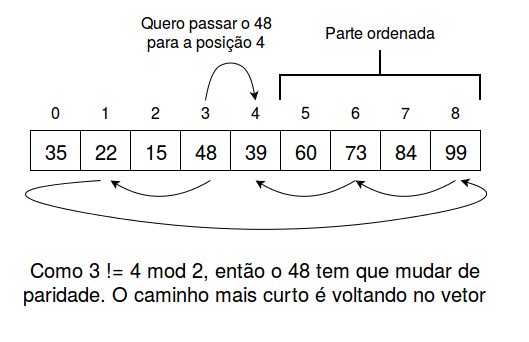
\includegraphics[scale=0.49]{vector13.png}\\
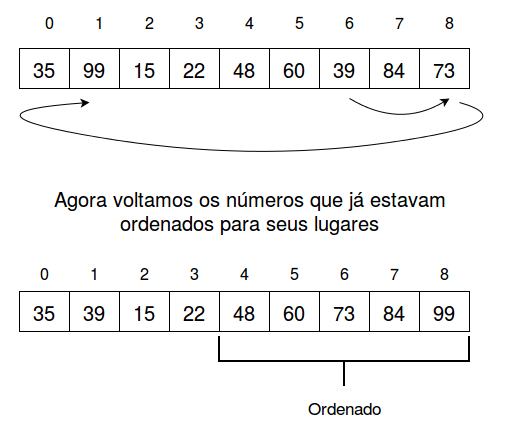
\includegraphics[scale=0.49]{vector23.png}\\
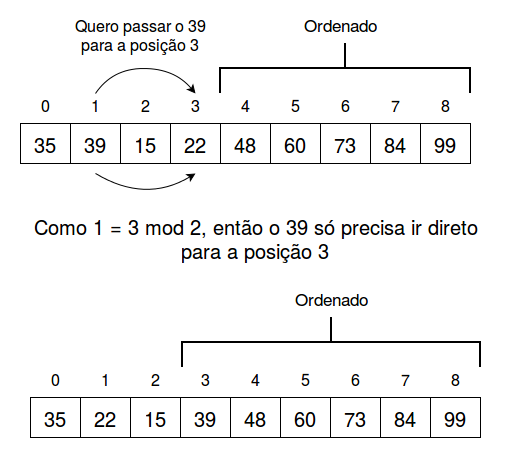
\includegraphics[scale=0.49]{vector32.png}\\
\end{center}
\normalsize
Como sempre é possível ordenar vetores ímpares, já que um número pode ir para qualquer posição do vetor, o programa imprime os movimentos feitos à medida que eles vão acontecendo.\\
Para vetores com um número par de posições, como não importa qual rotação seja feita, a paridade da posição de um elemento não muda, separei os números com índices pares e ímpares em dois vetores menores e os ordenei com um algoritmo de ordenação tradicional (nesse caso é utilizado o merge sort), já que nesses vetores uma 2-rotação é equivalente à uma 3-rotação no vetor original. Como é possível que o vetor seja impossível de ordenar, já que um número não pode ir para qualquer posição do vetor, o programa realiza dois merge sorts, o primeiro identifica se o vetor pode ser ordenado, se ele conseguir ordenar o vetor ele realizao o segundo sort para verificar quais movimentos o algoritmo fez e imprimi-los, caso contrário, ele imprime "Nao e possivel".\\[0.5cm]
\large
\item[5.]\textbf{Desempenho nos testes}
\normalsize\\[0.5cm]
Funcionou para todos os testes , sendo os maiores deles um vetor de $60.001$ posições, que demorou $95s$ para ser ordenado, um de $15.001$ posições no pior caso que demorou $10s$ e um de $60.000$, que demorou $30s$ (os tempos foram calculados colocando a saída do programa em um arquivo).\\[0.5cm]
\large
\item[6.]\textbf{Prós e contras}
\normalsize\\[0.5cm]
Prós:
\begin{itemize}
\item Ordena vetores pares em ordem O($n\log{n}$) no pior caso, pois utiliza um merge sort;
\item Dos muitos casos de teste realizados, o algoritmo funcionou para todos eles.
\end{itemize}
Contras:
\begin{itemize}
\item Também tem complexidade O($n\log{n}$) para vetores pares já ordenados, por utilizar o merge sort, e complexidade O($n^2$) no pior caso para vetores ímpares, já que ele faz $\frac{(n-1)^2}{2}$ movimentos e $\frac{n(n-1)}{2}$ comparações;
\item O algoritmo de ordenação para ímpares não é muito eficiente, por isso ele pode não achar os melhores movimentos que ordenam o vetor.
\end{itemize}
\end{enumerate}
\end{document}